% ===========================================================================
% Section 4: Test Setups
% ===========================================================================
\section{Test Setups}
\label{sec:test-setups}

This section describes the test setups used to investigate the research questions defined in Section~\ref{sec:research-questions}.
Each test setup specifies the devices under test, physical topology, traffic generation method, and measurement protocol.
\todo{Add introductory paragraph linking test design philosophy (automated, reproducible, phased).}

% ---------------------------------------------------------------------------
\subsection{Test~1: Incremental Port Load Test (Completed)}
\label{sec:test-incremental-port-load}
% ---------------------------------------------------------------------------

This test investigates how power consumption changes as Ethernet ports are incrementally loaded with maximum UDP traffic.
It directly addresses \textbf{RQ1} (power vs.\ number of active ports) and provides partial data for \textbf{RQ4} (idle power suitability for continuous operation) and \textbf{RQ8} (rated vs.\ real-world maximum power).

\subsubsection{Devices Under Test}
Four devices were tested, representing a range of consumer and ISP-provided equipment:
\begin{description}
    \item[Fritzbox 7530] (2018, 802.11ac, 4$\times$ GbE LAN, rated 18\,W max)
    \item[Asus RT-AX68U] (2020, 802.11ax, 4$\times$ GbE LAN, rated 33\,W max)
    \item[Huawei EchoLife EG8245W5-8T] (2020, 802.11ax, 4$\times$ GbE LAN, rated 24\,W max)
    \item[Alcatel HH40V] (2018, 802.11n, 2$\times$ 100\,Mbps LAN, rated 10\,W max)
\end{description}

\subsubsection{Physical Topology}
Figure~\ref{fig:test1_topology} shows the physical test setup.
The PC (equipped with a 4-port 2.5\,GbE NIC) connects 1--4 Ethernet cables to the device under test (DUT), which is powered through the DECT~200 smart plug for power measurement.
A \emph{separate} Fritzbox~7530 (not under test) hosts the DECT~200 base station and provides the TR-064 API endpoint for reading power data.
This isolation is critical: under heavy CPU load, the DUT's management API becomes unresponsive, which would cause measurement gaps if the DUT itself were used for data collection.

\begin{figure}[H]
    \centering
    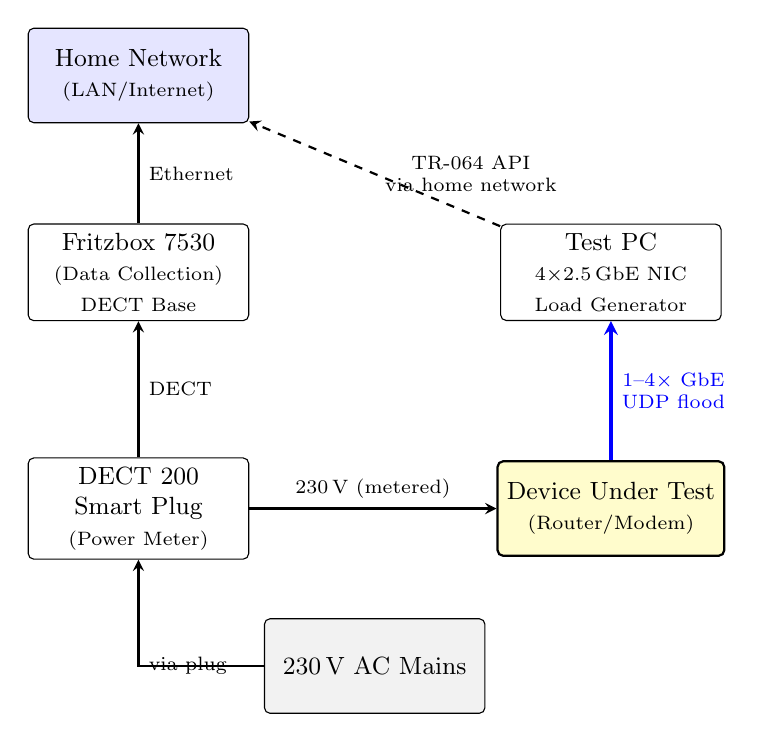
\begin{tikzpicture}[
        box/.style={rectangle, draw, minimum width=2.8cm, minimum height=1.2cm, text centered, font=\small, align=center, rounded corners=2pt},
        dut/.style={box, fill=yellow!20, thick},
        arrow/.style={->, >=stealth, thick},
        dashedarrow/.style={->, >=stealth, thick, dashed},
        lbl/.style={font=\scriptsize, midway, align=center}
    ]
        % Power Meter
        \node[box] (meter) at (0,0) {DECT~200\\Smart Plug\\{\scriptsize (Power Meter)}};

        % Data Collection Fritzbox
        \node[box] (fritzbox) at (0,3) {Fritzbox 7530\\{\scriptsize (Data Collection)}\\{\scriptsize DECT Base}};

        % Device Under Test
        \node[dut] (dut) at (6,0) {Device Under Test\\{\scriptsize (Router/Modem)}};

        % Main PC
        \node[box] (pc) at (6,3) {Test PC\\{\scriptsize 4$\times$2.5\,GbE NIC}\\{\scriptsize Load Generator}};

        % Home Network
        \node[box, fill=blue!10] (network) at (0,5.5) {Home Network\\{\scriptsize (LAN/Internet)}};

        % AC Power
        \node[box, fill=gray!10] (mains) at (3,-2) {230\,V AC Mains};

        % Connections
        \draw[arrow] (meter) -- node[right, lbl] {DECT} (fritzbox);
        \draw[arrow] (fritzbox) -- node[right, lbl] {Ethernet} (network);
        \draw[dashedarrow] (pc) -- node[right, lbl] {TR-064 API\\{\scriptsize via home network}} (network);
        \draw[arrow] (mains) -| node[near end, right, lbl] {via plug} (meter);
        \draw[arrow] (meter) -- node[above, lbl] {230\,V (metered)} (dut);
        \draw[arrow, very thick, blue] (dut) -- node[right, lbl, text=blue] {1--4$\times$ GbE \\{\scriptsize UDP flood}} (pc);

    \end{tikzpicture}
    \caption{Physical topology for the Incremental Port Load Test. The DUT is powered through the DECT~200 smart plug. A separate Fritzbox handles power data collection via DECT and TR-064.}
    \label{fig:test1_topology}
\end{figure}

\subsubsection{Test Protocol}
Each device was tested using the following automated protocol, executed by the custom web application described in Section~\ref{sec:automation}:
\begin{enumerate}
    \item \textbf{Pre-test baseline} (10\,min): All Ethernet cables connected but no traffic generated. Measures idle power with active link-up on all ports.
    \item \textbf{Load phase~1} (20\,min): Maximum UDP flood on \textbf{1~port} (target: 1\,Gbps).
    \item \textbf{Load phase~2} (20\,min): Maximum UDP flood on \textbf{2~ports} (target: 2\,Gbps).
    \item \textbf{Load phase~3} (20\,min): Maximum UDP flood on \textbf{3~ports} (target: 3\,Gbps). \emph{Skipped for Alcatel~HH40V (only 2 ports).}
    \item \textbf{Load phase~4} (20\,min): Maximum UDP flood on \textbf{4~ports} (target: 4\,Gbps). \emph{Skipped for Alcatel.}
    \item \textbf{Post-test baseline} (20\,min): All traffic stopped, cables remain connected. Measures power recovery behavior.
\end{enumerate}

\noindent\textbf{Load generation parameters:}
\begin{itemize}
    \item Protocol: UDP, packet size: 1400\,bytes, 16 workers per interface
    \item Target: device's own IP address (e.g., \texttt{169.254.1.1:80} for Fritzbox)
    \item Interfaces activated incrementally with 5 ramp-up steps per interface
    \item Power polling interval: 5\,seconds (via TR-064 SOAP API)
\end{itemize}

\noindent\textbf{Important limitation:} Traffic is directed at the DUT's own IP address, meaning all packets are processed by the device's \emph{CPU/software stack}, not merely switched at Layer~2 by the switching ASIC. This represents a CPU-intensive workload (similar to heavy NAT processing or connection handling) rather than pure L2 forwarding. As a result, devices with weaker CPUs (notably the Fritzbox~7530) show throughput degradation at higher port counts due to CPU saturation, not switching fabric limitations.

\subsubsection{Research Questions Addressed}
\begin{description}
    \item[RQ1 (Fully addressed):] The test directly measures power at 0, 1, 2, 3, and 4 active loaded ports, providing a complete port-count vs.\ power profile for each device.
    \item[RQ4 (Partially addressed):] The 10-minute pre-test baseline provides idle power measurements (with cables connected) for all four devices, enabling an idle power comparison and annual energy cost estimation. A full 24-hour idle measurement is not captured.
    \item[RQ8 (Partially addressed):] By comparing the maximum observed power under full Ethernet load to the manufacturer's rated maximum, we can assess how close real-world usage comes to the rated specification. This test does not activate Wi-Fi or USB peripherals, so the absolute maximum is not reached.
\end{description}

% ---------------------------------------------------------------------------
\subsection{Test~2: Throughput Scaling and Link Speed (Planned)}
\label{sec:test-throughput-scaling}
% ---------------------------------------------------------------------------

This test combines two research questions into a single measurement campaign by varying both throughput level and link speed on a single Ethernet port.
It directly addresses \textbf{RQ2} (100\,Mbps vs.\ 1\,Gbps) and \textbf{RQ3} (power vs.\ throughput at intermediate load levels).

\subsubsection{Devices Under Test}
All four devices from Test~1. The Alcatel~HH40V (100\,Mbps ports) participates only in Run~B.

\subsubsection{Physical Topology}
The physical topology is identical to Test~1 (Figure~\ref{fig:test1_topology}): single Ethernet cable from test PC to DUT, power measured via DECT~200.
Figure~\ref{fig:test2_ramp_profile} shows the expected throughput profile for the ramp-step load generation.

\begin{figure}[H]
    \centering
    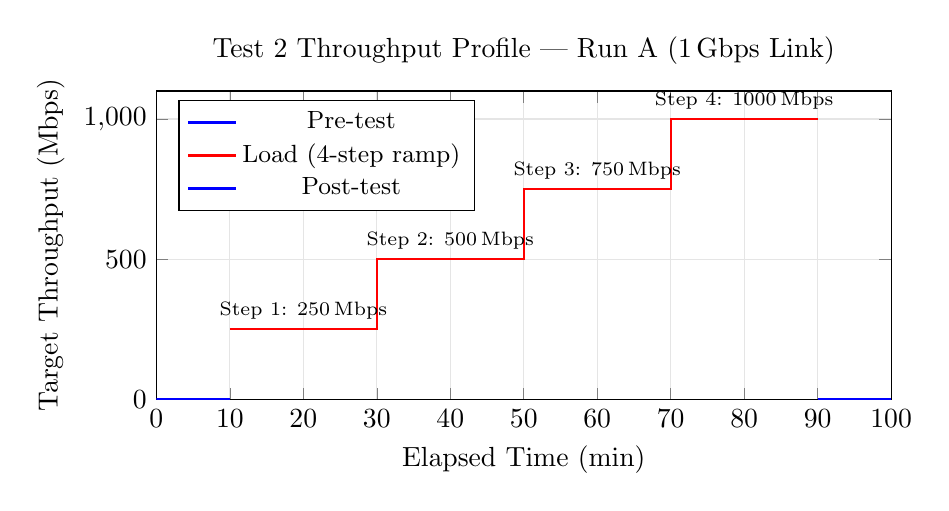
\begin{tikzpicture}
        \begin{axis}[
            width=0.90\linewidth,
            height=5.5cm,
            xlabel={Elapsed Time (min)},
            ylabel={Target Throughput (Mbps)},
            xmin=0, xmax=100,
            ymin=0, ymax=1100,
            grid=major,
            grid style={gray!20},
            title={Test~2 Throughput Profile --- Run~A (1\,Gbps Link)},
            legend pos=north west,
            legend style={font=\small},
        ]
            % Pre-test
            \addplot[blue, thick] coordinates {(0,0) (10,0)};
            \addlegendentry{Pre-test}
            % Ramp steps
            \addplot[red, thick] coordinates {(10,250) (30,250) (30,500) (50,500) (50,750) (70,750) (70,1000) (90,1000)};
            \addlegendentry{Load (4-step ramp)}
            % Post-test
            \addplot[blue, thick] coordinates {(90,0) (100,0)};
            \addlegendentry{Post-test}
            
            % Annotations
            \node[font=\scriptsize, anchor=south] at (axis cs:20,250) {Step 1: 250\,Mbps};
            \node[font=\scriptsize, anchor=south] at (axis cs:40,500) {Step 2: 500\,Mbps};
            \node[font=\scriptsize, anchor=south] at (axis cs:60,750) {Step 3: 750\,Mbps};
            \node[font=\scriptsize, anchor=south] at (axis cs:80,1000) {Step 4: 1000\,Mbps};
        \end{axis}
    \end{tikzpicture}
    \caption{Expected throughput profile for Test~2 Run~A. The load generator's ramp-step feature automatically transitions through four equal-duration steps. Run~B uses the same structure with 100\,Mbps maximum (steps at 25, 50, 75, 100\,Mbps).}
    \label{fig:test2_ramp_profile}
\end{figure}

\subsubsection{Test Protocol}
The test uses the load generator's built-in \emph{ramp steps} feature, which linearly increases the per-interface rate limit in equal increments.
Two runs are performed per device:

\paragraph{Run~A --- 1\,Gbps Link:}
\begin{enumerate}
    \item \textbf{Pre-test baseline} (10\,min): 1 cable connected, no traffic.
    \item \textbf{Load phase} (80\,min total): Single port, UDP, \texttt{ramp\_steps=4}, \texttt{target\_mbps=1000}.
    The load generator automatically steps through:
    \begin{itemize}
        \item Step~1 (20\,min): $\sim$250\,Mbps (25\% of link capacity)
        \item Step~2 (20\,min): $\sim$500\,Mbps (50\%)
        \item Step~3 (20\,min): $\sim$750\,Mbps (75\%)
        \item Step~4 (20\,min): $\sim$1000\,Mbps (100\%)
    \end{itemize}
    \item \textbf{Post-test baseline} (10\,min): Traffic stopped, cable remains connected.
\end{enumerate}

\paragraph{Run~B --- 100\,Mbps Link:}
Before starting, force the test PC's NIC to 100\,Mbps using Windows Device Manager or PowerShell:
\begin{verbatim}
    # PowerShell (run as Administrator):
    Set-NetAdapterAdvancedProperty -Name "Ethernet" `
        -DisplayName "Speed & Duplex" -DisplayValue "100 Mbps Full Duplex"
\end{verbatim}
Alternatively, use Device Manager $\rightarrow$ Network Adapters $\rightarrow$ Properties $\rightarrow$ Advanced $\rightarrow$ Speed \& Duplex $\rightarrow$ select \texttt{100 Mbps Full Duplex}.
Then repeat the same structure with \texttt{target\_mbps=100} and \texttt{ramp\_steps=4}, yielding steps at 25, 50, 75, and 100\,Mbps.
After completion, restore to auto-negotiation (typically 2.5\,Gbps on the Realtek controller):
\begin{verbatim}
    Set-NetAdapterAdvancedProperty -Name "Ethernet" `
        -DisplayName "Speed & Duplex" -DisplayValue "Auto Negotiation"
\end{verbatim}

\noindent\textbf{Load generation parameters (both runs):}
\begin{itemize}
    \item Protocol: UDP, packet size: 1400\,bytes, 16 workers
    \item Single interface enabled, \texttt{ramp\_duration} = 0 (auto, equals test duration)
    \item Target: DUT's own IP address (consistent with Test~1)
    \item Power polling interval: 5\,seconds
\end{itemize}

\subsubsection{Research Questions Addressed}
\begin{description}
    \item[RQ2 (Fully addressed):] Comparing idle power and power at matched throughput levels (e.g., 100\,Mbps via a 1\,GbE link vs.\ 100\,Mbps via a 100\,Mbps link) isolates the PHY-level power cost of the higher link speed.
    \item[RQ3 (Fully addressed):] The four-step ramp produces a power-vs-throughput curve at 25\%, 50\%, 75\%, and 100\% utilization for each link speed, revealing whether power scales linearly, sub-linearly, or in discrete steps.
\end{description}
\todo{Run this test and fill in results.}

% ---------------------------------------------------------------------------
\subsection{Test~3: Energy Efficiency and Extended Idle (Planned)}
\label{sec:test-energy-efficiency}
% ---------------------------------------------------------------------------

This test combines extended idle measurements with Energy-Efficient Ethernet (EEE, IEEE~802.3az) toggling to investigate both continuous-operation suitability and the real-world impact of power-saving features.
It directly addresses \textbf{RQ4} (idle power suitability) and \textbf{RQ6} (power-saving mode impact).

\subsubsection{Devices Under Test}
All four devices. EEE support will be verified per-device via \texttt{ethtool --show-eee} on connected ports.
Devices that do not support EEE will only undergo the extended idle portion.

\subsubsection{Physical Topology}
The physical topology is identical to Test~1 (Figure~\ref{fig:test1_topology}).
Figure~\ref{fig:test3_configurations} illustrates the three configuration variants.

\begin{figure}[H]
    \centering
    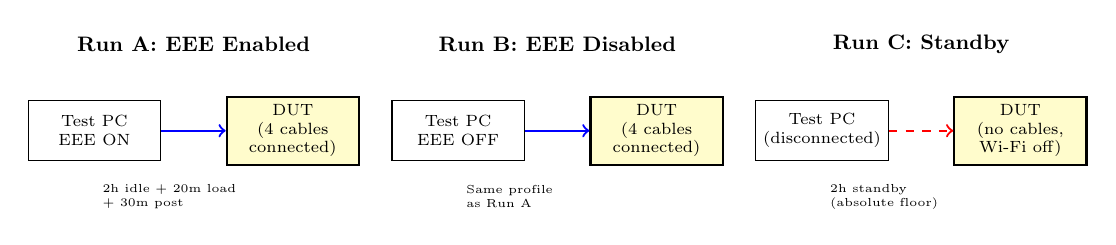
\begin{tikzpicture}[scale=0.84, transform shape,
        box/.style={rectangle, draw, minimum width=2.0cm, minimum height=0.9cm, text centered, font=\scriptsize, align=center},
        dut/.style={box, fill=yellow!20, thick},
        cable/.style={->, thick, blue},
        nocable/.style={->, thick, red, dashed},
    ]
        % Run A - EEE Enabled
        \node[font=\small\bfseries] at (0, 1.8) {Run A: EEE Enabled};
        \node[box] (pca) at (-1.5, 0.5) {Test PC\\EEE ON};
        \node[dut] (duta) at (1.5, 0.5) {DUT\\(4 cables\\connected)};
        \draw[cable] (pca) -- (duta);
        \node[font=\tiny, align=left, anchor=west] at (-1.5, -0.5) {2h idle + 20m load\\+ 30m post};
        
        % Run B - EEE Disabled
        \node[font=\small\bfseries] at (5.5, 1.8) {Run B: EEE Disabled};
        \node[box] (pcb) at (4, 0.5) {Test PC\\EEE OFF};
        \node[dut] (dutb) at (7, 0.5) {DUT\\(4 cables\\connected)};
        \draw[cable] (pcb) -- (dutb);
        \node[font=\tiny, align=left, anchor=west] at (4, -0.5) {Same profile\\as Run A};
        
        % Run C - No Cables
        \node[font=\small\bfseries] at (11, 1.8) {Run C: Standby};
        \node[box] (pcc) at (9.5, 0.5) {Test PC\\(disconnected)};
        \node[dut] (dutc) at (12.5, 0.5) {DUT\\(no cables,\\Wi-Fi off)};
        \draw[nocable] (pcc) -- (dutc);
        \node[font=\tiny, align=left, anchor=west] at (9.5, -0.5) {2h standby\\(absolute floor)};
    \end{tikzpicture}
    \caption{Test~3 configuration variants. Run~A and Run~B use the same physical setup but differ in EEE settings. Run~C disconnects all cables to measure true standby power.}
    \label{fig:test3_configurations}
\end{figure}

\subsubsection{Test Protocol}
Three runs are performed per device, requiring manual reconfiguration between runs:

\paragraph{Run~A --- EEE Enabled (Default):}
\begin{enumerate}
    \item Verify EEE is active: \texttt{ethtool --show-eee ethX} on the test PC.
    \item \textbf{Extended idle baseline} (2\,hours): All 4 cables connected, no traffic. Captures periodic background activity (DHCP renewal, Wi-Fi beaconing, firmware checks).
    \item \textbf{Load phase} (20\,min): 1 port, maximum UDP. Establishes a loaded power reference with EEE active.
    \item \textbf{Post-test recovery} (30\,min): Observe how quickly the device returns to idle power.
\end{enumerate}

\paragraph{Run~B --- EEE Disabled:}
\begin{enumerate}
    \item Disable EEE on test PC: \texttt{ethtool --set-eee ethX eee off}.
    \item If DUT exposes EEE settings (e.g., via admin UI), disable there as well.
    \item Repeat the same profile as Run~A (2\,h idle + 20\,min load + 30\,min post).
\end{enumerate}

\paragraph{Run~C --- Minimal Configuration (No Cables):}
\begin{enumerate}
    \item Disconnect all Ethernet cables from the DUT.
    \item Disable Wi-Fi via the DUT's admin interface (if possible).
    \item \textbf{Standby measurement} (2\,hours): Measures true standby power with no active interfaces.
\end{enumerate}

\noindent\textbf{Load generation parameters (Runs~A and B, load phase only):}
\begin{itemize}
    \item Protocol: UDP, packet size: 1400\,bytes, 16 workers, single interface
    \item \texttt{target\_mbps} = 0 (unlimited), no ramp steps
    \item Power polling interval: 5\,seconds
\end{itemize}

\subsubsection{Research Questions Addressed}
\begin{description}
    \item[RQ4 (Fully addressed):] The 2-hour idle measurements (with cables, without cables) provide a robust idle power characterization including any periodic background power fluctuations. Combined with the 10-minute baselines from Test~1, this enables confident annual energy cost projections and automated-shutdown recommendations.
    \item[RQ6 (Fully addressed):] Direct comparison of Run~A (EEE on) vs.\ Run~B (EEE off) at both idle and loaded states quantifies the real-world power savings from IEEE~802.3az. Run~C establishes the absolute floor.
\end{description}
\todo{Run this test and fill in results.}

% ---------------------------------------------------------------------------
\subsection{Test~4: Wi-Fi Impact and Maximum Load (Planned)}
\label{sec:test-wifi}
% ---------------------------------------------------------------------------

This test investigates the power cost of Wi-Fi by comparing Ethernet-only and Wi-Fi traffic paths, varying Wi-Fi band and distance, and finally combining all subsystems to approach the rated maximum power.
It addresses \textbf{RQ5} (Ethernet vs.\ Wi-Fi), \textbf{RQ7} (device type and signal strength), and completes \textbf{RQ8} (reaching rated maximum power).

\subsubsection{Devices Under Test}
Three devices with Wi-Fi: Fritzbox~7530 (802.11ac), Asus~RT-AX68U (802.11ax), Huawei~EG8245W5-8T (802.11ax).
The Alcatel~HH40V (802.11n, 2.4\,GHz only) may be included for a limited subset.

\subsubsection{Physical Topology}
Figure~\ref{fig:test4_wifi_topology} shows the physical setup for Runs~A--D (Wi-Fi traffic) and Run~E (combined Ethernet + Wi-Fi maximum load).

\begin{figure}[H]
    \centering
    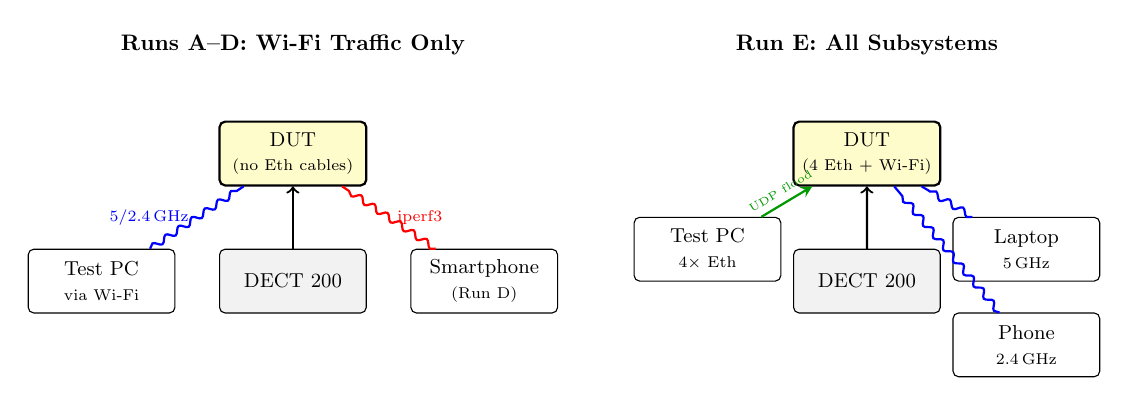
\begin{tikzpicture}[scale=0.81, transform shape,
        box/.style={rectangle, draw, minimum width=2.3cm, minimum height=1.0cm, text centered, font=\small, align=center, rounded corners=2pt},
        dut/.style={box, fill=yellow!20, thick},
        wifi/.style={decorate, decoration={snake, amplitude=0.4mm, segment length=2mm, post length=1mm}, thick, blue},
        eth/.style={->, >=stealth, thick, green!60!black},
    ]
        % Runs A-D: WiFi only
        \node[font=\bfseries] at (0, 4.2) {Runs A--D: Wi-Fi Traffic Only};
        \node[dut] (dut1) at (0, 2.5) {DUT\\{\scriptsize (no Eth cables)}};
        \node[box] (pc1) at (-3, 0.5) {Test PC\\{\scriptsize via Wi-Fi}};
        \node[box] (phone1) at (3, 0.5) {Smartphone\\{\scriptsize (Run D)}};
        \draw[wifi] (pc1) -- node[left, font=\scriptsize, midway] {5/2.4\,GHz} (dut1);
        \draw[wifi, red] (phone1) -- node[right, font=\scriptsize, midway] {iperf3} (dut1);
        \node[box, fill=gray!10] (meter1) at (0, 0.5) {DECT~200};
        \draw[->, thick] (meter1) -- (dut1);
        
        % Run E: Combined maximum
        \node[font=\bfseries] at (9, 4.2) {Run E: All Subsystems};
        \node[dut] (dut2) at (9, 2.5) {DUT\\{\scriptsize (4 Eth + Wi-Fi)}};
        \node[box] (pc2) at (6.5, 1) {Test PC\\{\scriptsize 4$\times$ Eth}};
        \node[box] (laptop2) at (11.5, 1) {Laptop\\{\scriptsize 5\,GHz}};
        \node[box] (phone2) at (11.5, -0.5) {Phone\\{\scriptsize 2.4\,GHz}};
        \draw[eth] (pc2) -- node[above, font=\tiny, sloped] {UDP flood} (dut2);
        \draw[wifi] (laptop2) -- (dut2);
        \draw[wifi] (phone2) -- (dut2);
        \node[box, fill=gray!10] (meter2) at (9, 0.5) {DECT~200};
        \draw[->, thick] (meter2) -- (dut2);
    \end{tikzpicture}
    \caption{Test~4 physical topologies. Runs~A--D use Wi-Fi-only traffic to isolate Wi-Fi power consumption. Run~E combines maximum Ethernet load (4 ports) with multiple Wi-Fi clients to approach the rated maximum power.}
    \label{fig:test4_wifi_topology}
\end{figure}

\subsubsection{Test Protocol}
Five runs are performed per device. Runs~A--D each follow the same structure: 10\,min idle, 20\,min load, 10\,min post.
The test PC connects to the DUT's Wi-Fi network and uses its Wi-Fi interface in the load generator.

\paragraph{Run~A --- Wi-Fi 5\,GHz, Near ($<$2\,m), Laptop:}
\begin{itemize}
    \item Test PC connected to DUT via 5\,GHz Wi-Fi (all Ethernet cables disconnected from DUT).
    \item Single Wi-Fi interface, UDP, \texttt{target\_mbps=0} (maximum achievable).
    \item 16 workers, 1400-byte packets.
\end{itemize}

\paragraph{Run~B --- Wi-Fi 2.4\,GHz, Near ($<$2\,m), Laptop:}
\begin{itemize}
    \item Same as Run~A but connected to the DUT's 2.4\,GHz SSID.
\end{itemize}

\paragraph{Run~C --- Wi-Fi 5\,GHz, Far ($\sim$10\,m, 1 wall), Laptop:}
\begin{itemize}
    \item Same as Run~A but with the test PC positioned $\sim$10\,m from the DUT, through one wall.
    \item Record signal strength (RSSI) at test start and end via \texttt{iwconfig} or \texttt{iw dev wlanX link}.
\end{itemize}

\paragraph{Run~D --- Wi-Fi 5\,GHz, Near, Smartphone:}
\begin{itemize}
    \item A smartphone runs \texttt{iperf3 -c <DUT\_IP> -u -b 0 -t 1200} as the traffic source instead of the custom load generator.
    \item The test application runs in power-monitoring-only mode (\texttt{load\_enabled = off}).
    \item Custom markers annotate the start/stop of the iperf3 session.
\end{itemize}

\paragraph{Run~E --- Combined Maximum Load (All Subsystems):}
This run attempts to reach the manufacturer's rated maximum power:
\begin{itemize}
    \item All 4 Ethernet ports loaded with maximum UDP (same as Test~1, 4-port phase).
    \item Simultaneously, 1--2 Wi-Fi clients connected and generating traffic (laptop on 5\,GHz, smartphone on 2.4\,GHz).
    \item If the DUT has a USB port, attach a USB storage device.
    \item Pre-test: 10\,min, combined load: 20\,min, post-test: 10\,min.
    \item The load generator runs on the test PC targeting all 4 Ethernet interfaces; Wi-Fi clients run independently.
\end{itemize}

\noindent\textbf{Ethernet baseline:} For RQ5 comparison, the single-port Ethernet results from Test~1 (load phase~1) serve as the Ethernet baseline, avoiding redundant measurements.

\subsubsection{Research Questions Addressed}
\begin{description}
    \item[RQ5 (Fully addressed):] Comparing Test~1 Ethernet-only power with Runs~A/B (Wi-Fi-only) at comparable throughput levels isolates the per-client power cost of each medium.
    \item[RQ7 (Fully addressed):] Runs~A vs.\ C (near vs.\ far) and Runs~A vs.\ D (laptop vs.\ smartphone) isolate the effects of distance/signal strength and client type on DUT power consumption.
    \item[RQ8 (Fully addressed):] Run~E loads all subsystems simultaneously, providing the closest approximation to the rated maximum. Combined with the Ethernet-only maximum from Test~1, this reveals how much power headroom the Wi-Fi radios and other peripherals account for.
\end{description}
\todo{Run this test and fill in results.}

% ---------------------------------------------------------------------------
\subsection{Test~5: ISP Bridge Mode Comparison (Planned)}
\label{sec:test-bridge-mode}
% ---------------------------------------------------------------------------

This test investigates whether splitting ISP-provided equipment into bridge mode plus a dedicated router reduces total system power consumption compared to using the ISP device in standalone router mode.
It directly addresses \textbf{RQ9}.

\subsubsection{Devices Under Test}
\begin{description}
    \item[Configuration~A (Standalone):] Huawei EG8245W5-8T operating as router (NAT, DHCP, Wi-Fi, firewall).
    \item[Configuration~B (Split):] Huawei EG8245W5-8T in bridge mode (minimal processing) + Asus RT-AX68U as dedicated router.
\end{description}

\subsubsection{Physical Topology}
Figure~\ref{fig:test5_bridge_topology} compares the two configurations.

\begin{figure}[H]
    \centering
    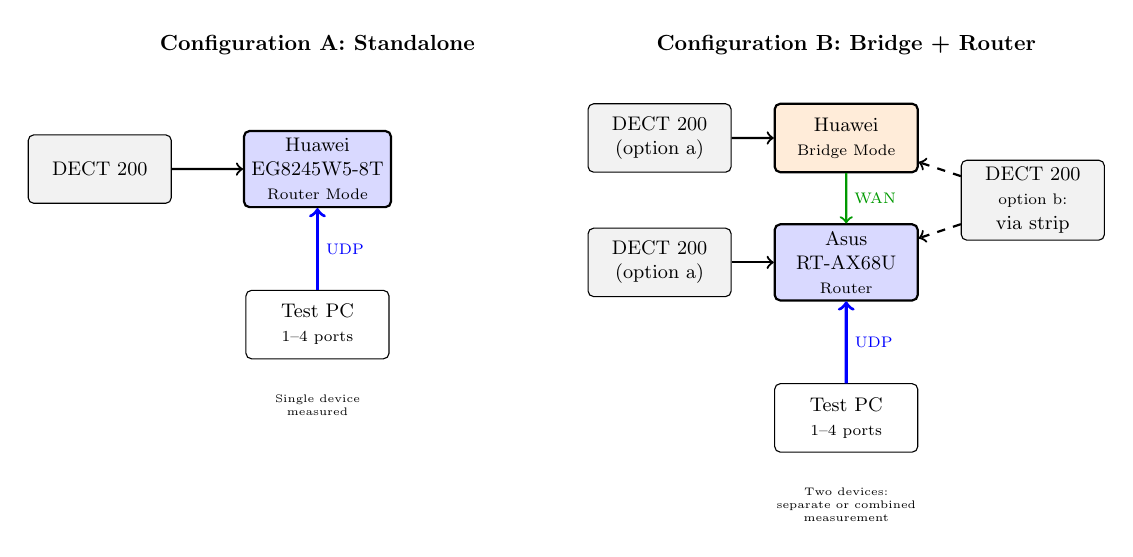
\begin{tikzpicture}[scale=0.79, transform shape,
        box/.style={rectangle, draw, minimum width=2.3cm, minimum height=1.1cm, text centered, font=\small, align=center, rounded corners=2pt},
        router/.style={box, fill=blue!15, thick},
        bridge/.style={box, fill=orange!15, thick},
        meter/.style={box, fill=gray!10},
    ]
        % Configuration A - Standalone
        \node[font=\bfseries] at (0, 5) {Configuration A: Standalone};
        \node[router] (huawei_a) at (0, 3) {Huawei\\EG8245W5-8T\\\scriptsize Router Mode};
        \node[box] (pc_a) at (0, 0.5) {Test PC\\\scriptsize 1--4 ports};
        \node[meter] (meter_a) at (-3.5, 3) {DECT~200};
        \draw[->, thick] (meter_a) -- (huawei_a);
        \draw[->, very thick, blue] (pc_a) -- node[right, font=\scriptsize] {UDP} (huawei_a);
        \node[font=\tiny, anchor=north, align=center] at (0, -0.5) {Single device\\measured};
        
        % Configuration B - Bridge Mode
        \node[font=\bfseries] at (8.5, 5) {Configuration B: Bridge + Router};
        \node[bridge] (huawei_b) at (8.5, 3.5) {Huawei\\\scriptsize Bridge Mode};
        \node[router] (asus_b) at (8.5, 1.5) {Asus\\RT-AX68U\\\scriptsize Router};
        \node[box] (pc_b) at (8.5, -1) {Test PC\\\scriptsize 1--4 ports};
        \node[meter] (meter_b1) at (5.5, 3.5) {DECT~200\\(option a)};
        \node[meter] (meter_b2) at (5.5, 1.5) {DECT~200\\(option a)};
        \node[meter] (meter_b_shared) at (11.5, 2.5) {DECT~200\\\scriptsize option b:\\via strip};
        
        \draw[->, thick] (meter_b1) -- (huawei_b);
        \draw[->, thick] (meter_b2) -- (asus_b);
        \draw[->, thick, dashed] (meter_b_shared) -- (huawei_b);
        \draw[->, thick, dashed] (meter_b_shared) -- (asus_b);
        \draw[->, thick, green!60!black] (huawei_b) -- node[right, font=\scriptsize] {WAN} (asus_b);
        \draw[->, very thick, blue] (pc_b) -- node[right, font=\scriptsize] {UDP} (asus_b);
        \node[font=\tiny, anchor=north, align=center] at (8.5, -2) {Two devices:\\separate or combined\\measurement};
    \end{tikzpicture}
    \caption{Test~5 topology comparison. Configuration~A uses the Huawei in full router mode. Configuration~B splits functionality: Huawei in bridge mode (pass-through) with Asus as the primary router. Power can be measured per-device (two DECT~200 plugs) or as a combined system (single plug via power strip).}
    \label{fig:test5_bridge_topology}
\end{figure}

\subsubsection{Test Protocol}
Both configurations are tested with the same incremental port load profile as Test~1 for direct comparability:
\begin{enumerate}
    \item \textbf{Pre-test baseline} (10\,min): Cables connected, no traffic.
    \item \textbf{Load phases} (4$\times$20\,min): Incremental 1--4 port UDP flood.
    \item \textbf{Post-test baseline} (10\,min): Traffic stopped.
\end{enumerate}

\paragraph{Configuration~A:} Standard Test~1 protocol on the Huawei.
A single DECT~200 smart plug measures total Huawei power.

\paragraph{Configuration~B:}
\begin{itemize}
    \item Huawei set to bridge mode via its admin interface (disables NAT, DHCP, firewall, optionally Wi-Fi).
    \item Asus RT-AX68U configured as the primary router (WAN port connected to Huawei's LAN port).
    \item Test PC connects to the Asus's LAN ports.
    \item \textbf{Power measurement:} Two options depending on available equipment:
    \begin{enumerate}
        \item[(a)] Two DECT~200 plugs (one per device) --- enables separate per-device power attribution.
        \item[(b)] Both devices on a single DECT~200 via a power strip --- measures combined system power directly.
    \end{enumerate}
\end{itemize}

\noindent\textbf{Load generation parameters:} Identical to Test~1 (UDP, 1400\,bytes, 16 workers, 5\,s polling).

\subsubsection{Research Questions Addressed}
\begin{description}
    \item[RQ9 (Fully addressed):] Comparing Configuration~A total power vs.\ Configuration~B total power (Huawei bridge + Asus router) at each load level reveals whether the bridge-mode split is more or less efficient. The per-device breakdown (if two plugs are available) shows how much power the Huawei saves in bridge mode vs.\ how much the Asus adds.
\end{description}
\todo{Run this test and fill in results.}
